\section{Empirical Evaluation}
\label{sec:evaluation}

We present the empirical evaluation of seventy-two algorithm-queue combinations on the Moscow road network. 
First, we analyze execution time composition using our multivariate OLS regression. 
Second, we validate performance significance with ANOVA. 
Third, we outline the three-step filtering pipeline to isolate the optimal configurations.

\subsection{Execution Latency Decomposition}

Our OLS regression models total routing latency $T_{\text{ms}}$ as a function of visited nodes, queue execution time, and priority pop cycles:
\begin{equation}
\begin{aligned}
T_{\text{ms}} = & 0.9921 - (8.46 \times 10^{-5}) \cdot N_{\text{visited}} \\
& + 3.3214 \cdot T_{\text{queue}} - 0.0082 \cdot C_{\text{pop}}
\end{aligned}
\label{eq:ols_formula}
\end{equation}
The regression results yield an R-squared value of 0.998 with an F-statistic of $2.041 \times 10^{5}$ ($p < 10^{-3}$). 
The positive coefficient of 3.3214 for $T_{\text{queue}}$ demonstrates that priority queue operations scale query latency. 
The negative coefficient for $C_{\text{pop}}$ reflects loop micro-optimizations that offset memory lookup delays. 

ANOVA results verify that the search algorithm, priority queue layout, and path edges exert significant impacts on total execution time. 
We record F-statistics of $F_{\text{Algorithm}} = 1305.63$, $F_{\text{Queue}} = 30.76$, and $F_{\text{PathEdges}} = 7691.36$ ($p < 10^{-40}$). 
These metrics confirm that priority queue selection dictates performance limits without regard to the topological routing parameters.

\subsection{The Three-Step Filtering Pipeline}

To identify the optimal routing configuration, we establish a three-step filtering pipeline that discards suboptimal search space and memory layout variants.

\subsubsection{Step 1: Algorithmic Filtering (Search Envelope Exponent)}
We isolate the relationship between path length $L$ and search latency $T_{\text{ms}}$ using a power-law model $T_{\text{ms}} = k \cdot L^{\alpha}$. 
Dijkstra routing explores a broad circular envelope, producing a complexity exponent of $\alpha = 2.0947$ ($R^2 = 0.7724$). 
A* search with $w=1.0$ exhibits directed search but suffers from high exploration width, yielding $\alpha = 2.4506$ ($R^2 = 0.8389$). 
In contrast, ALT routing with $w=1.0$ restricts the search space to a narrow corridor, achieving a complexity exponent of $\alpha = 1.8690$ ($R^2 = 0.4889$). 

Figure \ref{fig:complexity_elasticity} (Panel A) illustrates this microarchitectural isomorphism. 
The complexity exponents remain parallel across different queue backends, showing that the priority queue acts as a scaling constant while the search algorithm dictates the exponent $\alpha$. 
We filter out Dijkstra and A* due to their excessive search envelopes, leaving ALT as the candidate paradigm.

\subsubsection{Step 2: Accuracy and Re-opening Filtering}
We examine the impact of heuristic inflation by scaling the ALT search weight $w$ beyond 1.0. 
Figure \ref{fig:ghost_reopening} (Panel A) shows that scaling $w > 1.0$ triggers a node re-opening storm. 
At $w=1.0$, the re-opening index $\rho$ is near 1.10. 
At $w=1.20$, $\rho$ exceeds 1.15. 
This re-opening storm floods the priority queue with duplicate states. 

Figure \ref{fig:ghost_reopening} (Panel B) tracks the resulting ghost-node density. 
The SimdRadixHeap and SimdBucketQueue encounter massive memory pollution, with ghost densities climbing from 0.33 to 0.45. 
This pollution degrades throughput, producing negative throughput elasticity. 
Thus, we restrict the ALT algorithm to $w=1.0$ to guarantee monotonicity.

\subsubsection{Step 3: Hardware Stability Filtering}
We evaluate tail latency stability under priority queue load. 
Figure \ref{fig:hardware_strain} reports tail latency roughness ($p99 / p50$) and excess kurtosis. 
SimdQuickHeap exhibits high kurtosis values up to 112.63 and tail roughness factors. 
This variance arises from the instruction-level checks and branch mispredictions in the lazy sorting logic. 

In contrast, our cache-conscious Simd8AryHeap and the bucket-based SimdRadixHeap show stable, deterministic profiles. 
Simd8AryHeap records a roughness factor under 4.0. 
This stable footprint confirms that hardware-friendly layouts minimize performance jitter.

\subsection{Journey Profile Clustering}

K-Means clustering groups the 1500 benchmark runs into three spatial profiles based on edge count and route length. 
Table \ref{tab:qps_performance} summarizes queue throughput (QPS) across these profiles under ALT $w=1.0$.

For Localized Profile queries (Cluster 2, average length 12.3 km), SimdRadixHeap achieves 3147 QPS, outperforming Simd8AryHeap at 2620 QPS. 
In the Megalopolis Profile (Cluster 1, average length 43.7 km), execution time is dominated by queue operations. 
Here, SimdRadixHeap maintains 631 QPS, while Simd8AryHeap delivers 449 QPS. 
SimdQuickHeap drops to 499 QPS due to sorting overhead. 
These results confirm SimdRadixHeap as the optimal backend for monotone ALT queries.

\begin{figure}[t]
\centering
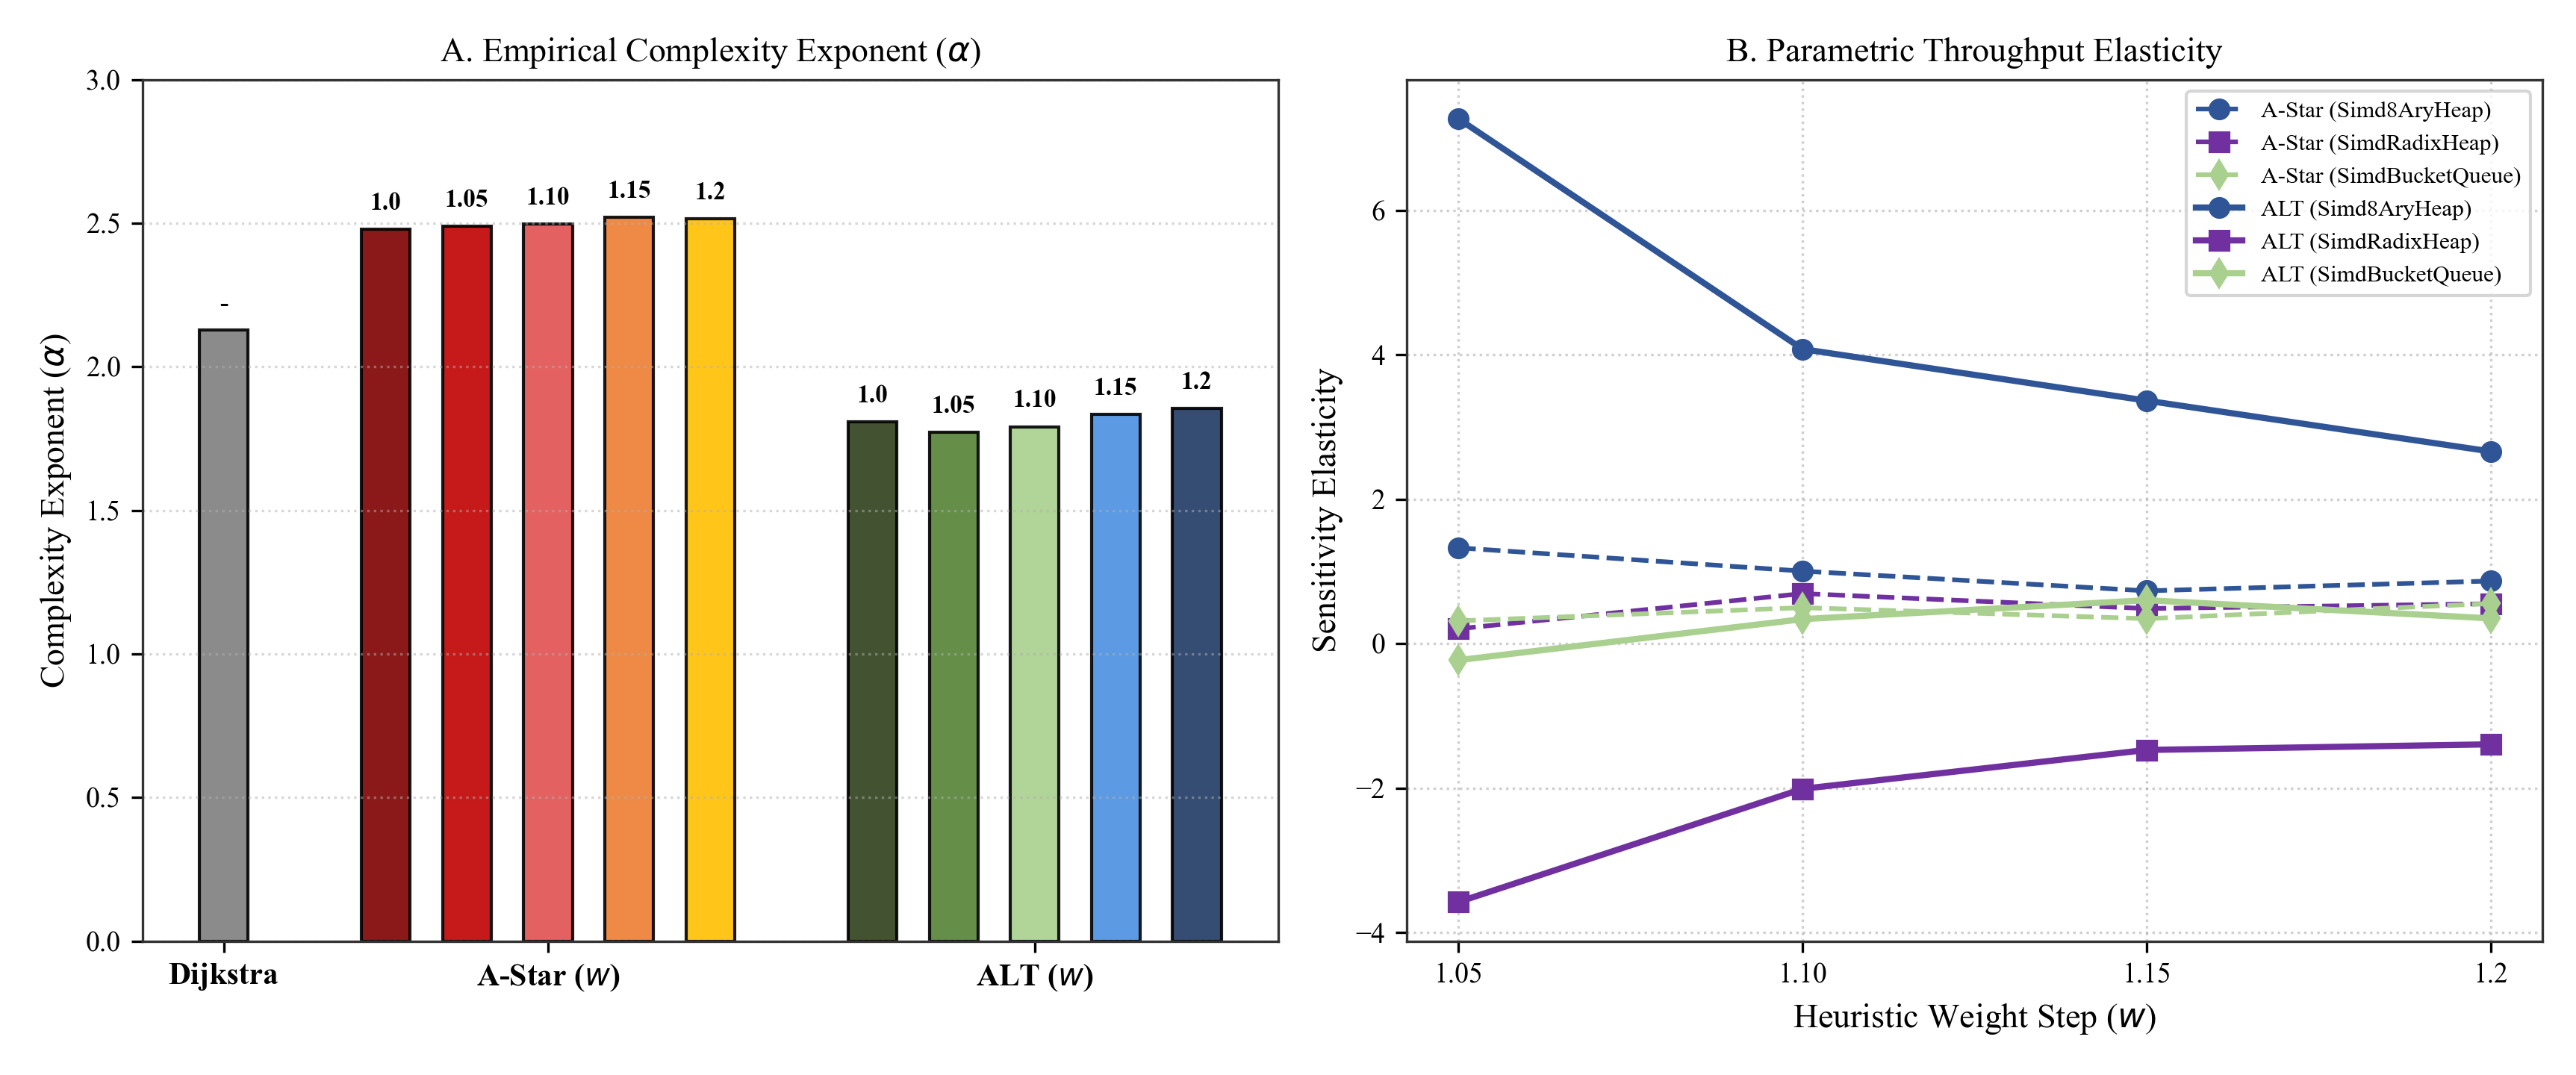
\includegraphics[width=\linewidth]{assets/complexity_elasticity_facets.png}
\caption{Complexity exponent $\alpha$ across algorithmic paradigms (Panel A) and parametric throughput elasticity under weight variations (Panel B).}
\label{fig:complexity_elasticity}
\end{figure}

\begin{figure}[t]
\centering
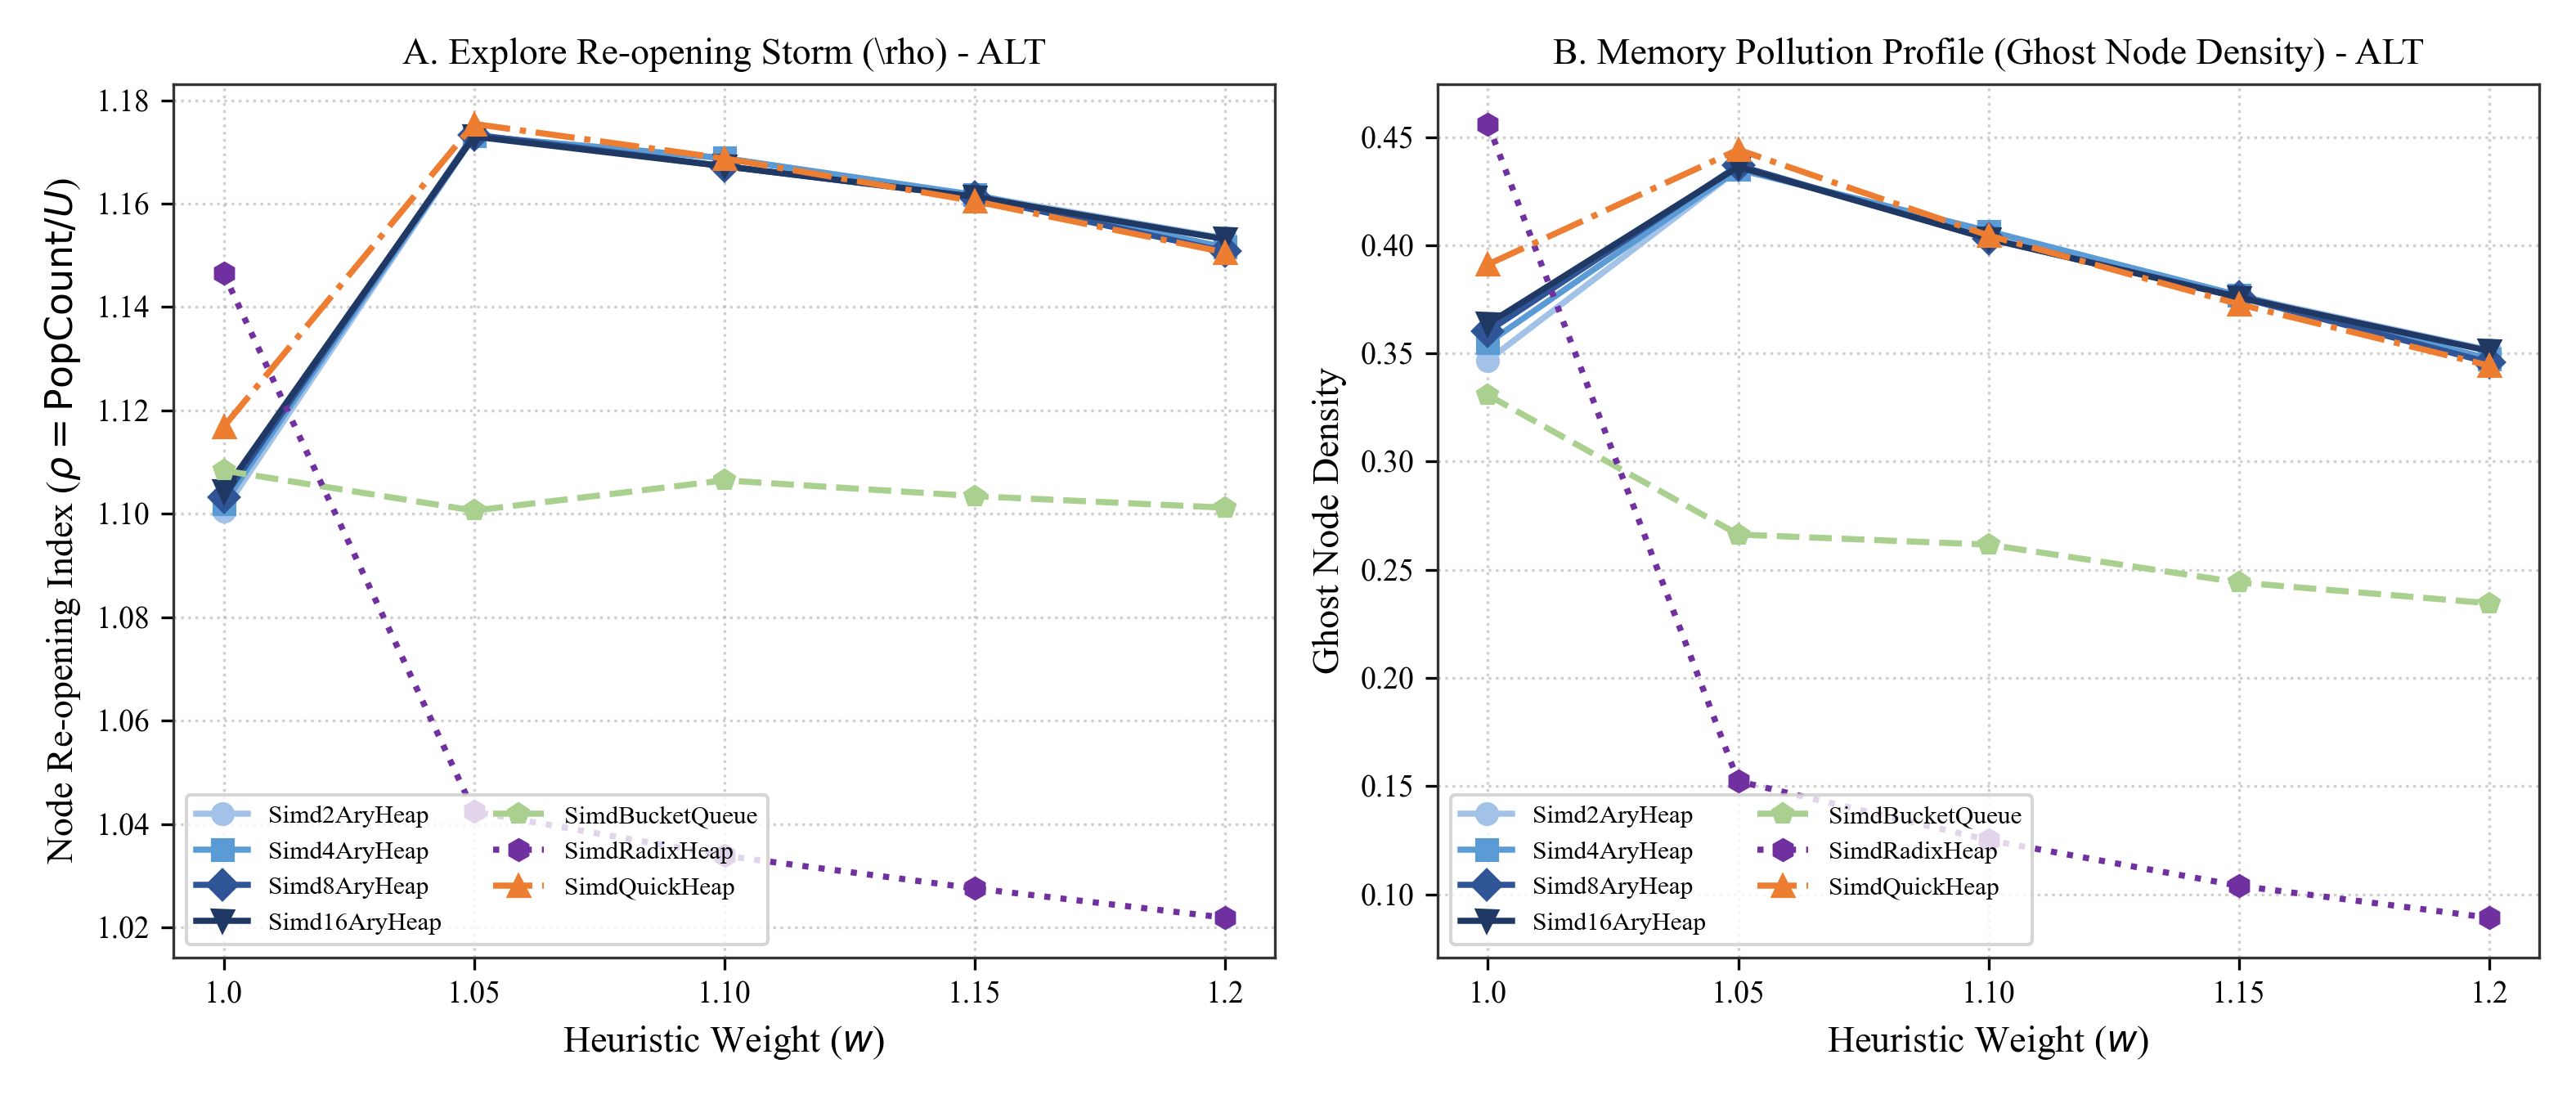
\includegraphics[width=\linewidth]{assets/ghost_reopening_cascade.png}
\caption{Node re-opening index $\rho$ (Panel A) and ghost-node memory pollution density (Panel B) as functions of heuristic weight $w$ under ALT routing.}
\label{fig:ghost_reopening}
\end{figure}

\begin{figure}[t]
\centering
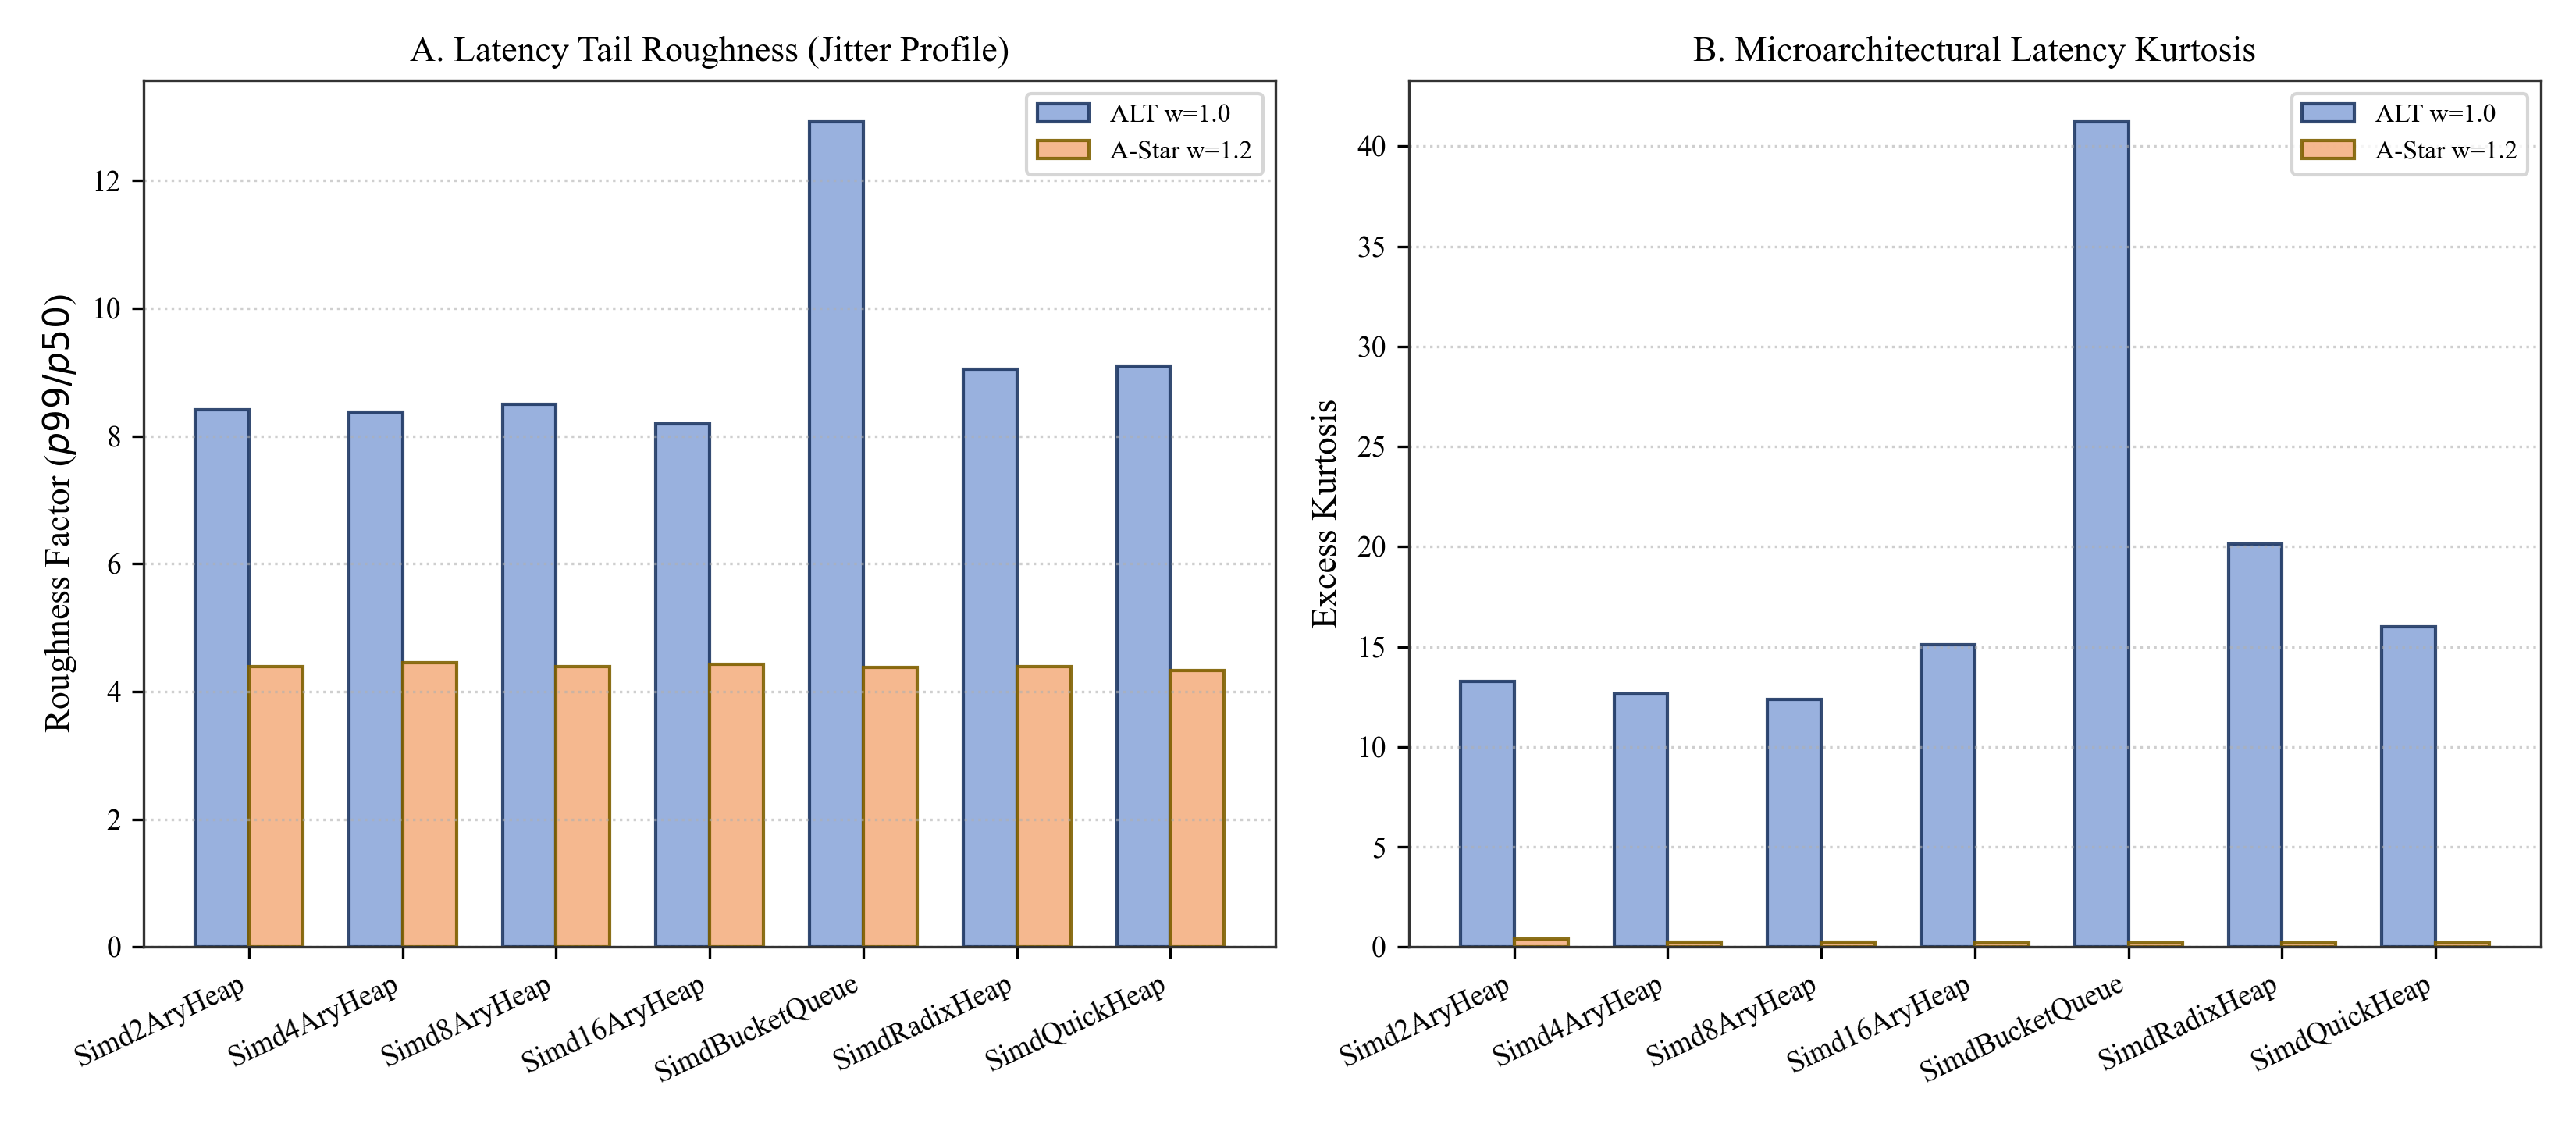
\includegraphics[width=\linewidth]{assets/hardware_strain_matrix.png}
\caption{Tail latency roughness factor (Panel A) and excess kurtosis (Panel B) illustrating microarchitectural hardware strain under queue execution noise.}
\label{fig:hardware_strain}
\end{figure}

\begin{table}[t]
\caption{Throughput (QPS) across K-Means Journey Clusters under ALT $w=1.0$}
\label{tab:qps_performance}
\centering
\begin{tabular}{lccc}
\toprule
\textbf{Queue Backend} & \textbf{Cluster 0 (Regional)} & \textbf{Cluster 1 (Megalopolis)} & \textbf{Cluster 2 (Localized)} \\
\midrule
Simd2AryHeap & 1516.99 & 429.46 & 2499.12 \\
Simd4AryHeap & 1554.19 & 444.35 & 2626.46 \\
Simd8AryHeap & 1594.81 & 449.11 & 2620.11 \\
Simd16AryHeap & 1558.92 & 451.93 & 2623.05 \\
SimdBucketQueue & 1819.85 & 569.30 & 2895.38 \\
SimdRadixHeap & 2007.87 & 631.57 & 3147.48 \\
SimdQuickHeap & 1690.49 & 499.99 & 2633.15 \\
\bottomrule
\end{tabular}
\end{table}
